
\chapter{Design}

\section{Requirements}

For this project, I will guarantee mutual isolation of tasks' stack and heap memory. Stack-allocated variables in one task shall not be readable nor writable by any other task. Similarly, memory allocated to a task on the heap will not be readable nor writable by any other task (until is freed and reallocated).

This implementation does not support process loading from disk (introduced in lab 5 of EE380L). All tasks are assumed to be compiled with the OS code, as is common for embedded RTOSes.

Importantly, this implementation does not protect task code. Tasks are able to execute any functions that they can be linked against.

Task memory will be protected automatically upon task creation and heap allocation.

As a proof of concept, my implementation can protect memory of up to sixteen different tasks. It cannot scale indefinitely. This is in part due to limitations of the MPU, which imposes a limit on the number of regions that can be individually configured. In a system that must support more tasks, the implementation could be changed to make protecting task memory optional, so that while only sixteen can be protected, more than that may run in the system at any given time.

\section{MPU Functionality}

The MPU is a hardware unit used to protect regions of memory. It supports up to eight configurable memory regions. Each region is configured with a base address, size, and permissions for both privileged and unprivileged access. The region's base address must be aligned to the size of the region. Each region is further divided into eight equally-sized subregions which can be individually enabled or disabled. My design will leverage subregions heavily to maximize the number of tasks that can be mutually isolated.

\section{Stack Protection}

Task stacks are allocated from a pool of statically allocated memory. Sixteen stacks each of 64 double words are declared to be allocated as tasks are created at runtime. Two consecutive MPU regions are initialized to span from the beginning of the stack pool up to the end. Using two regions allows us to evenly divide the pool into sixteen subregions each of which perfectly aligns with the boundaries of a single task stack. Therefore there is a one-to-one correspondence between MPU subregion and task ID. To protect the stack pool with the MPU, the stack pool must be aligned to the size of one of the MPU regions, which is $8\times64$ double words, or 4096 bytes.

\begin{figure}[hbtp]
	\centering
	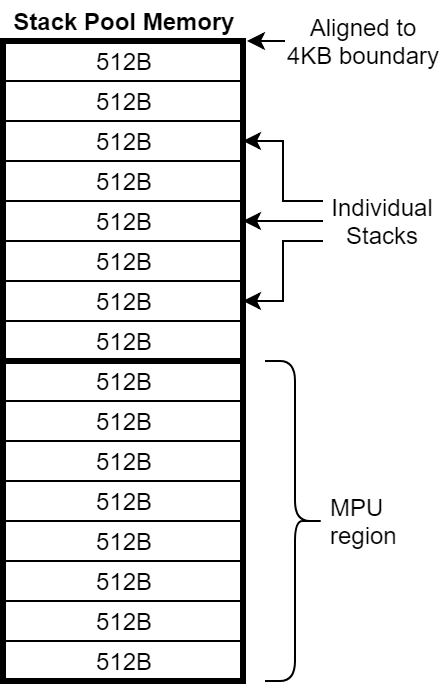
\includegraphics[width=0.4\columnwidth]{figs/stack_prot.png}
	\caption{Illustration of how the stack pool is organized in memory. Two consecutive MPU regions are configured to span the pool. The pool holds sixteen consecutive 512B stacks which each align with a MPU subregion. The whole stack pool is aligned to a 4KB boundary.}
	\label{fig:stack_prot}
\end{figure}
% https://www.draw.io/#G1K-jvmSFl7cc_w53rWbj7vP-SnMSNnW15

\section{Heap Protection}

The heap is implemented as a simple Knuth heap, based upon the implementation from lab 5, with some changes to accomodate the MPU. Any memory allocated to a task on the heap is guaranteed to be isolated from other tasks. This is achieved by grouping memory allocations together into MPU subregions by the owner task. When tasks are allocated memory, the heap manager associates the task's ID with all MPU subregions touched by the allocated block. The task now ``owns'' those subregions, and no other task will be allowed to acquire a block in those subregions. In this way, the heap manager guarantees that every subregion will contain blocks belonging to at most one task. At this point, protecting the heap is as simple as prohibiting access to heap subregions where the running task doesn't have any blocks.

A naive solution would be to statically partition the heap into sixteen pieces and allocate one to each task in the system. However, the approach I have chosen ought to scale better to systems where tasks may vary in their demand for heap memory. For example, if only eight out of sixteen tasks use the heap, then any blocks statically allocated to the other eight tasks would go unused -- a huge waste. In the case where there are sixteen tasks in the system and they each take turns acquiring heap memory, my solution will allocate each a subregion and converge to the simpler approach.

\begin{figure}[hbtp]
	\centering
	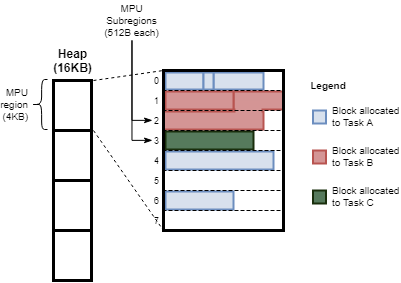
\includegraphics[width=0.7\linewidth]{figs/heap_prot.png}
	\caption{Illustration of how the heap is organized in memory. Two consecutive MPU regions are configured to span the heap, each with eight subregions. Memory allocated to different tasks will always be placed in different subregions such that every subregion's blocks are associated with at most one task. Allocated blocks are shown, color-coded according to which task requested them.}
	\label{fig:heap_prot}
\end{figure}
% https://www.draw.io/#G1K-jvmSFl7cc_w53rWbj7vP-SnMSNnW15

Figure \ref{fig:heap_prot} shows an example heap where three tasks have each been allocated memory. Each subregion will contain memory for at most one task. It's possible for a task's memory to span multiple subregions, as in subregions 1 and 2. This design is susceptible to some amount of internal and external fragmentation, though less than the naive solution I described earlier. You can see internal fragmentation at the end of subregion 0. Only small allocations can fit in the remaining free space of subregion 0, and they must be allocated to Task A to be put there in the first place (since Task A has claimed that subregion). As for external fragmentation, suppose Task C were to request 256 Bytes from the heap manager -- this is larger than one subregion. For that reason, the allocation \textit{could not} fit in the empty subregion 5. It would instead be placed in subregions 7 and 8, leaving subregion 5 to go to waste until a small enough block could be allocated there.

\section{Changes to TCB and Context Switch}

The TCB is expanded to include two masks which encode the stack and heap subregions the task is allowed to access. These additions are italicized in Listing \ref{lst:tcb}.

\begin{lstlisting}[language=c, caption={TCB struct definition}, captionpos=b, label={lst:tcb}]
typedef struct _tcb_s {
    long *sp;
    struct _tcb_s *next;
    uint32_t wake_time;
    unsigned long id;
    uint8_t priority;
    uint32_t period;
    unsigned long magic;
    void (*task)(void);
    char * task_name;
    pcb_t *parent_process;
    (*@\textit{unsigned int stack\_prot\_msk;}@*)
    (*@\textit{unsigned int heap\_prot\_msk;}@*)
} tcb_t;
\end{lstlisting}

During a context switch, the OS configures the MPU to allow access only to stack and heap subregions associated with the next running task. All other subregions (either associated with other tasks or unused) are protected.

\section{Final MPU Region Configuration}

Given the design described, MPU regions are configured as in Figure \ref{table:mpu_cfg}

\begin{table}[H]
    \begin{tabular}{|l|l|l|l|l|l|}
    \hline
    \multirow{2}{*}{\textbf{}} & \multirow{2}{*}{\textbf{Base}} & \multirow{2}{*}{\textbf{Size}} & \multicolumn{2}{l|}{\textbf{Access}}        & \multirow{2}{*}{\textbf{Notes}}                                                   \\ \cline{4-5}
                               &                                &                                & \textbf{Unprivileged} & \textbf{Privileged} &                                                                                   \\ \hline
    0                          & 0x00000000                     & 4GB                            & R/W                   & R/W                 & \begin{tabular}[c]{@{}l@{}}Allow access\\ if no other\\ rule applies\end{tabular} \\ \hline
    1                          & 0x00000000                     & 32B                            & None                  & None                & \begin{tabular}[c]{@{}l@{}}Catch null\\ pointer\end{tabular}                      \\ \hline
    2                          &                                &                                &                       &                     &                                                                                   \\ \hline
    3                          &                                &                                &                       &                     &                                                                                   \\ \hline
    4                          & \texttt{\&Heap}                & 1KB                            & None                  & None                & \begin{tabular}[c]{@{}l@{}}Heap\\ region 0\end{tabular}                           \\ \hline
    5                          & \texttt{\&Heap} + 1KB          & 1KB                            & None                  & None                & \begin{tabular}[c]{@{}l@{}}Heap\\ region 1\end{tabular}                           \\ \hline
    6                          & \texttt{\&Stack\_Pool}         & 4KB                            & None                  & None                & \begin{tabular}[c]{@{}l@{}}Stack pool\\ region 0\end{tabular}                     \\ \hline
    7                          & \texttt{\&Stack\_Pool} + 4KB   & 4KB                            & None                  & None                & \begin{tabular}[c]{@{}l@{}}Stack pool\\ region 1\end{tabular}                     \\ \hline
    \end{tabular}
    \caption{MPU Region Configutation.}
    \label{table:mpu_cfg}
\end{table}

